\documentclass{standalone}

\usepackage{tikz}
\usepackage{amssymb}
\usetikzlibrary{calc, positioning}
\begin{document}
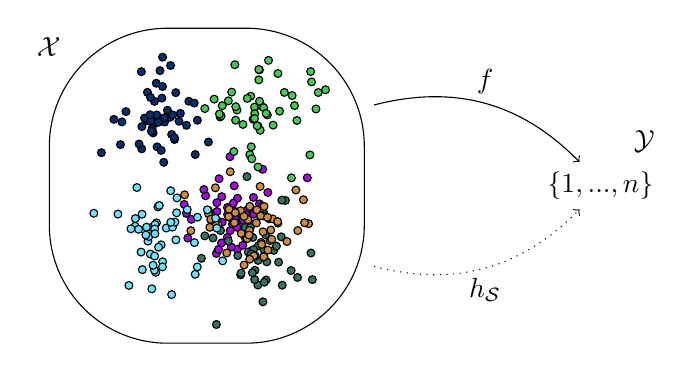
\begin{tikzpicture}
	\pgfmathsetseed{123}
	\draw[rounded corners = 1.5cm] (-2,-2) -- (-2,2) -- (2,2) -- (2,-2) -- cycle;
	\node (x1) at (2,1) {};
	\node (x2) at (2,-1) {};
	\node[below] at (current bounding box.north west) {$ \mathcal{X} $};

	\foreach \x in {1,...,6} {
			\pgfmathparse{rnd}
			\edef\red{\pgfmathresult}
			\pgfmathparse{rnd}
			\edef\green{\pgfmathresult}
			\pgfmathparse{rnd}
			\edef\blue{\pgfmathresult}
			\definecolor{groupColor}{rgb}{\red, \green, \blue}
			\begin{scope}[shift={(rand, rand)}]
				\foreach \x in {1,...,50}{
						\filldraw[fill=groupColor] ({rnd*rand}, {rnd*rand}) circle (0.05);
					}
			\end{scope}
		}

	\begin{scope}[xshift=5cm]
		\node[label={above right:$\mathcal{Y}$}] (y) at (0,0) {$ \{ 1,...,n \} $};
	\end{scope}

	\draw[->, bend left] (x1) to node[midway, above] {$ f $} (y);
	\draw[->, bend right, dotted] (x2) to node[midway, below] {$ h_{\mathcal{S}} $} (y);

\end{tikzpicture}
\end{document}
